\begin{figure*}[t]
  \centering
  \begin{subfigure}[t]{0.48\textwidth}
    \centering
    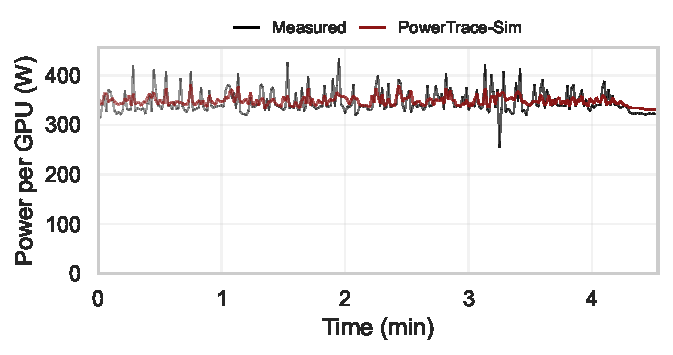
\includegraphics[width=\linewidth]{results/paper/appendix/power_trace_qwen3_14b_a100_tp1_dense_transfer_1s.pdf}
    \caption{Retrospective idle-calibrated dense transfer to unseen Qwen3-14B
    on A100 TP1. Pure request-only zero-shot transfer has
    4.62\% energy error. The shown trace
    keeps the frozen timing law and every dynamic power coefficient, replacing
    only the source idle floor (70.1~W/GPU)
    with the declared 60-second pre-request target idle
    (87.9~W/GPU). No loaded-target power sample
    enters the prediction. It reaches
    0.52\% energy error, 0.111 range
    NRMSE, and 0.0114 normalized Soft-DTW. The mean
    transfers, but ACF $R^2=-1.54$ shows that high-frequency
    event alignment does not. Because the idle update was applied after the
    sealed result was inspected, it is diagnostic rather than a sealed
    zero-shot claim.}
    \label{fig:qwen-dense-transfer}
  \end{subfigure}\hfill
  \begin{subfigure}[t]{0.48\textwidth}
    \centering
    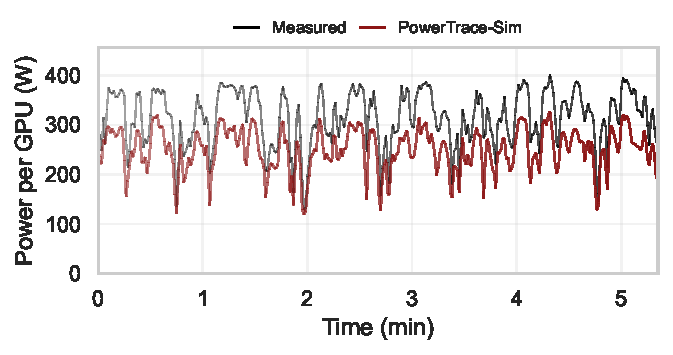
\includegraphics[width=\linewidth]{results/paper/appendix/power_trace_qwen3_30b_a3b_h100_tp2_moe_transfer_1s.pdf}
    \caption{Retrospective calibrated MoE transfer to unseen Qwen3-30B-A3B on
    H100 TP2. Pure GPT-OSS-20B zero-shot transfer has
    32.00\% energy error. The
    shown trace changes only the idle intercept to the pre-request 60-second
    target measurement (118.3~W/GPU) and rescales the frozen memory and
    compute terms by source-only H100/A100 energy-per-work ratios
    (0.916 and
    0.875). No loaded-target coefficient
    is fit. Energy error falls to 20.63\%, with
    0.254 NRMSE, 0.0362 Soft-DTW,
    and ACF $R^2=0.945$. Because this rule was selected after the
    sealed trace was inspected, it is diagnostic rather than a sealed claim.}
    \label{fig:qwen-moe-transfer}
  \end{subfigure}
  \caption{Architecture-aware transfer of PowerTrace-Sim to unseen dense and
  MoE checkpoints. Black is measured power and red is the request-generated
  prediction; both are matched nonoverlapping one-second per-GPU means over
  the complete common observation interval.}
  \label{fig:qwen-transfer-traces}
\end{figure*}
